\documentclass[11pt, a4paper]{article}

\usepackage{style}

\institution{EPFL}
\project{Semester Project}
\title{Minimal Rational Interpolation for Time-Harmonic Maxwell's Equations}
\author{Fabio Matti}
\supervisor{Prof. Fabio Nobile \\ Dr. Davide Pradovera}
\date{\today}

\begin{document}

\maketitle

\section*{Abstract}
\label{sec:abstract}

\pagebreak
\tableofcontents

\pagebreak
\section{Introduction}
\label{sec:introduction}

\pagebreak
\section{Finite element discretization of the time-harmonic Maxwell's equations}
\label{sec:maxwell}

\subsection{Vector potential formulation of the time-harmonic Maxwell's equations}
\label{subsec:maxwell-potential}

% !REMINDME: Add boundary conditions to th equations!!!!

% Everything smooth enough to do all manipulations...

Let $\mathbf{E}$ denote an electric field, $\mathbf{B}$ a magnetic field
strength, $\rho$ an electric charge density, and $\mathbf{j}$ an electric
current density. Maxwell's equations are stated in \citep{monk} as
\begin{align}
    \nabla \cdot (\epsilon \mathbf{E}) &= \rho \label{equ:maxwell1} \\
    \nabla \cdot \mathbf{B} &= 0 \label{equ:maxwell2} \\
    \nabla \times \mathbf{E} &= -\partial_t \mathbf{B} \label{equ:maxwell3} \\
    \nabla \times (\mu^{-1} \mathbf{B}) &= \partial_t (\epsilon \mathbf{E}) + \mathbf{j} \label{equ:maxwell4}
\end{align}
with $\varepsilon$ being the permittivity and $\mu$ the permeability.

% Non-conducting material, else => j = sigma*E + J_a (Monk 21)

Equation (\ref{equ:maxwell2}) allows for an expression of the magnetic field 
$\mathbf{B} = \nabla \times \mathbf{u}$ in terms of a vector valued function
$\mathbf{u}$, the vector potential (in literature commonly denoted with
$\mathbf{A}$). Similarly, (\ref{equ:maxwell3}) suggests
rewriting the electric field $\mathbf{E} = - \nabla \phi - \partial_t \mathbf{u}$
using a scalar function $\phi$, referred to as the scalar potential.

The physical quantities $\mathbf{E}$ and $\mathbf{B}$ remain unchanged 
if we transform $\mathbf{u} \to \mathbf{u}' = \mathbf{u} + \nabla \psi$ or
$\phi \to \phi' = \phi - \partial_t \psi$ for arbitrary functions $\psi$.
A convenient choice of $\psi$ is suggested in \citep{gauge-transformation} to be
\begin{equation}
    \psi = \int_0^t \phi dt' \label{equ:gauge}
\end{equation}
which transforms $\phi \to \phi' = 0$ and $\mathbf{u} \to \mathbf{u}' = \mathbf{u}
+ \nabla \int_0^t \phi dt'$. Thus, the expressions for the electrical and
magnetic field become
\begin{align}
    \mathbf{E} &= -\partial_t \mathbf{u} \label{equ:electricfield} \\
    \mathbf{B} &= \nabla \times \mathbf{u} \label{equ:magneticfield}
\end{align}
where I renamed the variable $\mathbf{u}'$ to $\mathbf{u}$ for simplicity.

Plugging the identities (\ref{equ:electricfield}) and (\ref{equ:magneticfield})
into (\ref{equ:maxwell4}) yields 
\begin{equation}
    \nabla \times (\mu^{-1} \nabla \times \mathbf{u}) =  \epsilon \partial_t^2 \mathbf{u} + \mathbf{j} \label{equ:maxwell-potential}
\end{equation}

For the rest of this report, I restrict myself to vector potentials $\mathbf{u}$
that exhibit a harmonic dependence on time $t$, i.e. may be factorized into
a term solely depending on the position $\mathbf{x}$ and a complex exponential
\begin{equation}
    \mathbf{u}(\mathbf{x}, t) = \mathbf{u}(\mathbf{x}) \exp(i \omega t) \label{equ:time-harmonic}
\end{equation}
Substituting this expression into (\ref{equ:maxwell-potential}) results in the
\begin{fancybox}{Time-harmonic potential equation}
    \begin{equation}
     \nabla \times (\mu^{-1} \nabla \times \mathbf{u}) - \epsilon \omega^2 \mathbf{u} = \mathbf{j} \label{equ:maxwell-timeharmonic}
    \end{equation}
\end{fancybox}

\subsection{Weak formulation for the time-harmonic potential equation}
\label{subsec:maxwell-weak}

Equation (\ref{equ:maxwell-timeharmonic}) may be multiplied by a vector-valued
function $\mathbf{v} \in H_{\textrm{curl}}(\Omega)$, where
\begin{equation}
    H_{\textrm{curl}}(\Omega) = \{\mathbf{u} : \Omega \to \mathbb{C},~\text{such that}~\mathbf{u}\in L^2(\mathbb{C})^3, \nabla \times \mathbf{u} \in L^2(\mathbb{C})^3\} \label{equ:h-curl}
\end{equation}
and then integrated over all of $\Omega$ to obtain 
\begin{equation}
    \int_{\Omega} (\nabla \times ({\mu^{-1} \nabla \times \mathbf{u}})) \cdot \mathbf{v}
    - \omega^2 \int_{\Omega} \epsilon \mathbf{u} \cdot \mathbf{v} = \int_{\Omega} \mathbf{j} \cdot \mathbf{v} \label{equ:maxwell-weak-initial}
\end{equation}
% !REMINDME: Put derivation in appendix
This may further be simplified (\ref{equ:maxwell-weak-initial}) to (see Section 
\ref{sec:abstract} for details)
\begin{fancybox}{Weak formulation of the time-harmonic potential equation}
    \begin{equation}
        \int_{\Omega} ({\mu^{-1} \nabla \times \mathbf{u}}) \cdot (\nabla \times \mathbf{v})
        - \omega^2 \int_{\Omega} \epsilon \mathbf{u} \cdot \mathbf{v} 
        = \int_{\Omega} \mathbf{j} \cdot \mathbf{v}
        + \int_{\partial \Omega} \underbrace{(({\mu^{-1} \nabla \times \mathbf{u}}) \times \mathbf{n})}_{= \mathbf{g}} \cdot \mathbf{v}
        \label{equ:maxwell-weak}
    \end{equation}
\end{fancybox}
where $\mathbf{n}$ denotes the surface normal to the boundary $\partial \Omega$.

Boundary conditions on the electric field $\mathbf{E}$ may be enforced in a Dirichlet-type
fashion through the relation (\ref{equ:electricfield}) and the assumption
(\ref{equ:time-harmonic})
\begin{equation}
    \left.\mathbf{u}\right|_{\partial \Omega} = -\frac{1}{i\omega} \left.\mathbf{E}\right|_{\partial \Omega} \label{equ:dirichlet-boundary}
\end{equation}
Those on the magnetic field $\mathbf{B}$ through a Neumann-type condition following
from (\ref{equ:magneticfield}) and again (\ref{equ:time-harmonic})
\begin{equation}
    \left.\mathbf{g}\right|_{\partial \Omega} = (\mu^{-1} \left.\mathbf{B}\right|_{\partial \Omega}) \times \mathbf{n} \label{equ:neumann-boundary}
\end{equation}

\subsection{Examples}
\label{subsec:examples}

We apply this weak formulation to three different but very intimately related 
problems:

\begin{figure}[h]
    \centering
    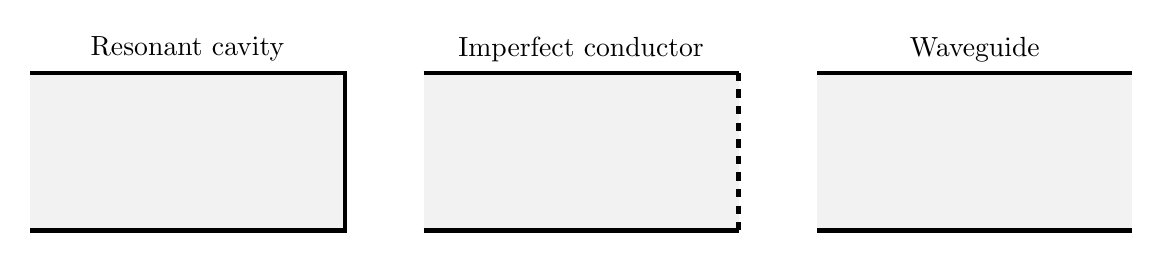
\begin{tikzpicture}
    \node at (2, 2.3) {Resonant cavity};
    \fill[black!5!white] (0, 0) rectangle (4, 2);
    \draw[ultra thick] (0, 0) to (4, 0) to (4, 2) to (0, 2);

    \node at (7, 2.3) {Imperfect conductor};
    \fill[black!5!white] (5, 0) rectangle (9, 2);
    \draw[ultra thick] (5, 0) to (9, 0);
    \draw[ultra thick, dashed] (9, 2) to (9, 0);
    \draw[ultra thick] (5, 2) to (9, 2);

    \node at (12, 2.3) {Waveguide};
    \fill[black!5!white] (10, 0) rectangle (14, 2);
    \draw[ultra thick] (10, 0) to (14, 0);
    \draw[ultra thick] (10, 2) to (14, 2);
\end{tikzpicture}
    \caption{Schematically the most trivial case for each example.}
    \label{fig:examples}
\end{figure}

\subsubsection{Two-dimensional resonant cavity}
\label{subsubsec:cavity}

A resonant cavity is a region $\Omega$ enclosed by a boundary $\partial \Omega$.
The boundary is subdivided into one (or more) inlets $\Gamma_N$ and a perfect
electrically conducting wall $\Gamma_D = \partial \Omega \setminus \Gamma_N$.

\begin{figure}[h]
    \centering
    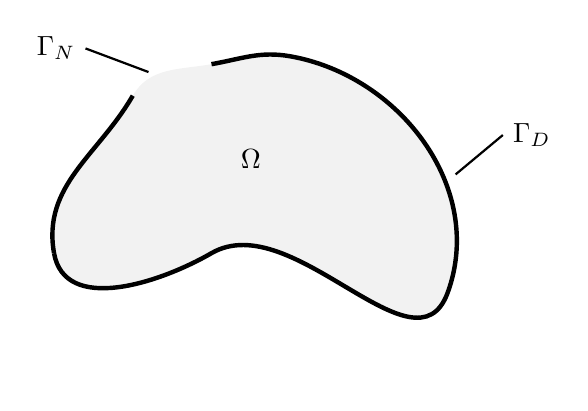
\begin{tikzpicture}
    \fill[black!5!white] (2, 1) to [out=100, in=240] (3, 3)
                              to [out=60, in=190] (4, 3.4)
                              to [out=10, in=170] (5, 3.5)
                              to [out=350, in=70] (7, 0.5)
                              to [out=250, in=30] (4, 1)
                              to [out=210, in=280] (2, 1);
    \draw[ultra thick] (2, 1) to [out=100, in=240] (3, 3);

    \draw[ultra thick] (4, 3.4) to [out=10, in=170] (5, 3.5)
                              to [out=350, in=70] (7, 0.5)
                              to [out=250, in=30] (4, 1)
                              to [out=210, in=280] (2, 1);
    \draw[thick] (2.4, 3.6) node[left] {$\Gamma_N$} to (3.2, 3.3);
    \draw[thick] (7.7, 2.5) node[right] {$\Gamma_D$} to (7.1, 2);
    \node at (4.5, 2.2) {$\Omega$};
\end{tikzpicture}
    \caption{2d resonant cavity.}
    \label{fig:2d-cavity}
\end{figure}

% !REMINDME: Why only need test against v_z?!
Suppose the current density $\mathbf{j} \equiv 0$ and orient the coordinate
system in such a way that $\mathbf{u} = u_z \mathbf{e}_z$ and 
$\mathbf{v} = v_z \mathbf{e}_z$. Consequently,
\begin{equation}
    (\mu^{-1} \nabla \times \mathbf{u}) \cdot (\nabla \times \mathbf{v})
    = (\mu^{-1} \nabla u_z) \cdot (\nabla v_z)
\end{equation}
Use $g_z = (\mathbf{g})_z$ along the boundary $\Gamma_N$,
to convert (\ref{equ:maxwell-weak}) into
the weak formulation for a two-dimensional resonant cavity
\begin{equation}
    \int_{\Omega} (\mu^{-1} \nabla u_z) \cdot (\nabla v_z)
    - \omega^2 \int_{\Omega} \epsilon u_z v_z
    = \int_{\partial \Omega} g_z v_z \label{equ:maxwell-weak-resonant-cavity}
\end{equation}

% Boundary conditions Dirichlet and Neumann (from Monk)
Let $\mathbf{E}$ and $\mathbf{B}$ refer to the electric and magnetic fields inside
the cavity. For now, I distinguish two types of boundaries.

For the perfectly conducting boundary, treated in \citep{monk}, it holds that
\begin{equation}
    \mathbf{n} \times \mathbf{E} = 0,~~\text{on}~\Gamma_D
\end{equation}
For the boundaries in a two-dimensional resonant cavity (see Figure 
\ref{fig:2d-cavity}), this only holds true if $E_z = 0$, which translates
to the Dirichlet boundary condition $\left.\mathbf{u}\right|_{\Gamma_D} = 0$
in light of (\ref{equ:dirichlet-boundary}).

For the inlet, it is easiest to enforce the boundary condition through the
magnetic field $\mathbf{B}$ (considering $\mathbf{n} = -\mathbf{e}_x$ as
depicted in Figure \ref{fig:2d-cavity}):
\begin{equation}
    g_z = (({\mu^{-1} \mathbf{B}}) \times (-\mathbf{e}_x))_z = \mu^{-1} B_x
\end{equation}

\subsubsection{Imperfect conductor}
\label{subsubsec:impedance}

% Additionally impedance boundary condition from Monk
At an imperfect boundary \cite{monk}, (\ref{equ:electricfield}), with (\ref{equ:time-harmonic})
\begin{equation}
    \mathbf{g} = (\mu^{-1} \nabla \times \mathbf{u}) \times \mathbf{n}
    = i \omega \lambda (\mathbf{n} \times \mathbf{u}) \times \mathbf{n}
\end{equation}
which, supposing that $\mathbf{u} = u_z \mathbf{e}_z$ and only treating a
two-dimensional domain, simplifies (using the fact that $\mathbf{n} \perp \mathbf{u}$
and $||\mathbf{n}|| = 1$, so $(\mathbf{n} \times \mathbf{u}) \times \mathbf{n} = \mathbf{u}$)
% !REMINDME: Maybe proof it in appendix
\begin{equation}
    g_z = i \omega \lambda u_z
\end{equation}
Therefore, reuse (\ref{equ:maxwell-weak-resonant-cavity}) as it is, but split 
boundary integral term for Neumann and impedance boundary.

\subsubsection{Waveguide}
\label{subsubsec:waveguide}

We go back to (\ref{equ:maxwell-weak}). Again, $\mathbf{j} \equiv 0$, but now 
we stay in 3d. Supposing that the inlet is located at a constant $x$-value,
such that the surface normal to this inlet is $-\mathbf{e}_x$. For an incoming
magnetic field $\left.\mathbf{B}\right|_{\Gamma_N} = B_0 \mathbf{e}_y$ at the
inlet, we see from (\ref{equ:neumann-boundary}) that $\left.\mathbf{g}\right|_{\Gamma_i}
= - \mu^{-1} B_0 \mathbf{e}_z$. At the outlet, we set $\left.\mathbf{g}\right|_{\Gamma_o} = \boldsymbol{0}$

% Just j=0 and 3d, need to discuss boundary conditions


\pagebreak
\section{Finite element approximation with FEniCS}
\label{sec:fem}

\subsection{Theory (come up with better title)}
\label{subsec:fem-theory}

% Theory

Along the lines of \cite{fenics}.

% WHAT SPACE DO WE WANT V TO BE?!?!
See immediately that the weak formulation (\ref{equ:maxwell-weak}) assumes the shape
\begin{equation}
    \text{Find}~\mathbf{u} \in V,~\text{such that}~a_{\omega}(\mathbf{u}, \mathbf{v}) = L(\mathbf{v}), ~\forall \mathbf{v} \in V_0
\end{equation}
with the bilinear form 
\begin{equation}
    a_{\omega}(\mathbf{u}, \mathbf{v}) = \int_{\Omega} (\mu^{-1} \nabla \times \mathbf{u}) \cdot (\nabla \times \mathbf{v})
    - \omega^2 \int_{\Omega} \epsilon \mathbf{u} \cdot \mathbf{v}
\end{equation}
and the linear form 
\begin{equation}
    L(\mathbf{u}) = \int_{\Omega} \mathbf{j} \cdot \mathbf{v} + \int_{\partial \Omega} \mathbf{g} \cdot \mathbf{v}
\end{equation}

% TO BE CONTINUED WITH GALERKIN STUFF

\subsection{Demonstration (come up with better title)}
\label{subsec:fem-demo}

% Demonstration
In the style of \cite{fenics}. 
Problem (\ref{equ:maxwell-weak}) with $\Omega$ being a cubic cavity with an inlet
on one side and all other sides with $\mu = \epsilon = 0$, $\mathbf{j} = 0$
for simplicity.

Required packages
\lstinputlisting[firstnumber=0, firstline=0, lastline=3]{code/fenics_example.py}

Mesh
\lstinputlisting[firstnumber=5, firstline=6, lastline=7]{code/fenics_example.py}

Function space (Nédélec elements of the first kind \cite{monk})
\lstinputlisting[firstnumber=9, firstline=10, lastline=10]{code/fenics_example.py}

Inlet (at x = 0)
\lstinputlisting[firstnumber=12, firstline=13, lastline=15]{code/fenics_example.py}

PEC boundary
\lstinputlisting[firstnumber=17, firstline=18, lastline=20]{code/fenics_example.py}

Boundary ids
\lstinputlisting[firstnumber=22, firstline=23, lastline=26]{code/fenics_example.py}

Dirichlet boundary (0 for PEC, because Nédélec)
\lstinputlisting[firstnumber=28, firstline=29, lastline=30]{code/fenics_example.py}

Neumann boundary (1 for ...)
\lstinputlisting[firstnumber=32, firstline=33, lastline=34]{code/fenics_example.py}

Trial and test functions
\lstinputlisting[firstnumber=36, firstline=37, lastline=38]{code/fenics_example.py}

Neumann boundary integral term
\lstinputlisting[firstnumber=40, firstline=41, lastline=41]{code/fenics_example.py}

Stiffness matrix
\lstinputlisting[firstnumber=43, firstline=44, lastline=45]{code/fenics_example.py}

Mass matrix
\lstinputlisting[firstnumber=47, firstline=48, lastline=49]{code/fenics_example.py}

L2 norms
\lstinputlisting[firstnumber=51, firstline=52, lastline=54]{code/fenics_example.py}

Solution at frequencies
\lstinputlisting[firstnumber=56, firstline=57, lastline=62]{code/fenics_example.py}

Plotting the L2-norms
\lstinputlisting[firstnumber=64, firstline=65, lastline=66]{code/fenics_example.py}

% Nédelec elements

\pagebreak
\section{Minimal rational interpolation for the time-harmonic Maxwell's equations}
\label{sec:mri}

% General idea 
Let $u : \mathbb{R} \to \mathbb{C}$.
Given $u_j = u(\omega_j)$ for $j \in \{1, \dots, S\}$. Want to find a surrogate
\begin{equation}
    \tilde{u}(\omega) \approx u(\omega)
\end{equation}

\subsection{Motivation}
\label{subsec:motivation}

Equations of the type (\ref{equ:maxwell-timeharmonic}), in the most simple case (dropping
all constants)
\begin{equation}
    \nabla \times (\nabla \times \mathbf{u}) - \omega^2 \mathbf{u} = \mathbf{j}
\end{equation}
Writing the double-curl operator in terms of a matrix $\mathbf{\underline{A}}$
\begin{equation}
    \mathbf{u} = (\mathbf{\underline{A}} - \omega^2)^{-1} \mathbf{j}
\end{equation}
Eigenvalue decomposition $\mathbf{\underline{A}} = \mathbf{\underline{V}} ~ \boldsymbol{\underline{\Lambda}} ~ \mathbf{\underline{V}}^H$
leads us to a form proposed in \cite{helmholtz-motivation}
\begin{equation}
    \mathbf{u} = \mathbf{\underline{V}} (\boldsymbol{\underline{\Lambda}} - \omega^2 \boldsymbol{\underline{1}})^{-1} \mathbf{\underline{V}}^H \mathbf{j} 
    = \sum_i \frac{\mathbf{v}_i \mathbf{v}_i^H \mathbf{j}}{\lambda_i - \omega^2} \label{equ:motivation}
    %= \sum_i \frac{\mathbf{r}_i}{\lambda_i - \omega^2} \label{equ:motivation}
\end{equation}
which follows from the fact that $\boldsymbol{\underline{\Lambda}}$ is diagonal,
hence also $(\boldsymbol{\underline{\Lambda}} - \omega^2 \boldsymbol{\underline{1}})^{-1}$.
Here, we denoted the diagonal elements of $\boldsymbol{\underline{\Lambda}}$ with 
$\lambda_i$ (the eigenvalues of $\mathbf{\underline{A}}$) and the columns of
$\mathbf{\underline{V}}$ with $\mathbf{v}_i$ (the eigenvectors of $\mathbf{\underline{A}}$).

% !REMINDME: This is not really phrased academically yet...
Hence, it would make sense to search for an approximation of the solution $\mathbf{u}$
that is able to \enquote{model} the singularities at $\omega^2 = \lambda_i$, e.g.
rational polynomials
\begin{equation}
    \tilde{u}(\omega) = \frac{P(\omega)}{Q(\omega)}
\end{equation}

% Algorithm (last column SVD is definition of MRI, cite Davide)
\citep{greedyMRI}

\begin{algorithm}
    \caption{Minimal rational interpolation} \label{alg:MRI}
    \begin{algorithmic}
    \Require $\omega_1, \dots, \omega_S$
    \Require $U = [u(\omega_1) | \dots | u(\omega_S)]$ \Comment{Snapshot matrix}
    \State Compute $G$ with $g_{ij} = \langle u(\omega_i), u(\omega_j)\rangle_M,~ i, j \in \{1, \dots, S \}$ \Comment{Gramian matrix}
    \State Compute the singular value decomposition $G = V \Sigma V^H$
    \State Define $q = V[:, S]$
    \State Define $\tilde{u}(\omega) = P(\omega) / Q(\omega)$ with $P(\omega) = \sum_{j=1}^S \frac{q_j u(\omega_j)}{\omega - \omega_j}$ and $Q(\omega) = \sum_{j=1}^S \frac{q_j}{\omega - \omega_j}$
\end{algorithmic}
\end{algorithm}

\citep{shortMRI}

\begin{algorithm}
    \caption{Greedy minimal rational interpolation} \label{alg:gMRI}
    \begin{algorithmic}
    \Require $\tau > 0$ \Comment{Relative $L_2$-error tolerance}
    \Require $\Omega_{\mathrm{test}} = \{\omega_i\}_{i=1}^M$ \Comment{Set of candidate support points}
    \Require $a_{\omega}(\mathbf{u}, \mathbf{v}) = L(\mathbf{v})$ \Comment{Finite element formulation of the problem}
    \State Choose $\omega_1, \dots, \omega_t \in \Omega_{\mathrm{test}}$ \Comment{Usually the smallest and largest element}
    \State Remove $\omega_1, \dots, \omega_t$ from $\Omega_{\mathrm{test}}$
    \State Solve $a_{\omega_i}(\mathbf{u}_i, \mathbf{v}) = L(\mathbf{v})$ for $i \in \{1, \dots, t\}$
    \State Build surrogate $\mathbf{\tilde{u}}_t = \mathbf{P}_t(\omega) / Q_t(\omega)$ using the solutions $\mathbf{u}_1, \dots, \mathbf{u}_t$
    \While{$\Omega_{\mathrm{test}} \neq \emptyset$}
        \State $\omega_{t+1} \leftarrow \textrm{argmin}_{\omega \in \Omega_{\mathrm{test}}} |Q_t(\omega)|$
        \State Solve $a_{\omega_{t+1}}(\mathbf{u}_{t+1}, \mathbf{v}) = L(\mathbf{v})$
        \State Build surrogate $\mathbf{\tilde{u}}_{t+1} = \mathbf{P}_{t+1}(\omega) / Q_{t+1}(\omega)$ using the solutions $\mathbf{u}_1, \dots, \mathbf{u}_{t+1}$
        \If{$||\mathbf{u}_{t+1} - \mathbf{\tilde{u}}_{t}(\omega_{t+1})||_M / ||\mathbf{u}_{t+1}||_M < \tau$}
            \Return
        \EndIf
        \State $t \leftarrow t+1$
    \EndWhile
    %\Return $\tilde{A}(\omega) = \sum_i \frac{q_i A(\omega_i)}{\omega - \omega_i} / \sum_i \frac{q_i}{\omega - \omega_i}$
\end{algorithmic}
\end{algorithm}

% Interpolation property (in barycentric expansion, l'Hôpital whatever)
The rational surrogate $\mathbf{\tilde{u}}$ can be rewritten as 
\begin{align}
    \mathbf{\tilde{u}}(\omega)
    &= \sum_{j=1}^S \frac{q_j \mathbf{u}(\omega_j)}{\omega - \omega_j}
    / \sum_{j=1}^S \frac{q_j}{\omega - \omega_j} \notag \\
    &= \sum_{j=1}^S \prod_{\substack{i=0 \\ i \neq j}}^S (\omega - \omega_i) q_j \mathbf{u}(\omega_j)
    / \sum_{j=1}^S \prod_{\substack{i=0 \\ i \neq j}}^S (\omega - \omega_i) q_j
\end{align}
Therefore, if the rational surrogate $\mathbf{\tilde{u}}$ is evaluated at one of the
interpolation nodes $\omega_i$, $\mathbf{u}(\omega_i)$ is recovered.

If the rational surrogate $\mathbf{\tilde{u}}$ is evaluated in a zero
$\bar{\omega}$ of the denominator $Q(\bar{\omega}) = 0$, we observe a pole,
unless $P(\bar{\omega})$ happens to vanish too.

% Rational root finding 

\citep{klein}

Defining 
\begin{equation}
    v_i = (\omega - \omega_i)^{-1}
\end{equation}
and requiring
\begin{equation}
    0 = Q(\omega) = \sum_{i=1}^S q_i v_i(\omega)
\end{equation}
can be equivalently expressed as a generalized eigenvalue problem
\begin{equation}
    \mathbf{\underline{A}} \mathbf{u} = \omega \mathbf{\underline{B}} \mathbf{u}
\end{equation}
with
\begin{equation}
    \mathbf{\underline{A}} = \begin{pmatrix}
        0 & q_1 & q_2 & \dots & q_S \\
        1 & \omega_1 & & & \\
        1 & & \omega_2 & & \\ 
        \vdots & & & \ddots & \\ 
        1 & & & & \omega_S
    \end{pmatrix} ~~\text{and}~~
    \mathbf{\underline{B}} = \begin{pmatrix}
        0 & & & & \\
         & 1 & & & \\
         & & 1 & & \\ 
        \vdots & & & \ddots & \\ 
         & & & & 1
    \end{pmatrix}\label{equ:root-finding}
\end{equation}

% Optimization tweaks

% -> Householder sequential algorithm instead of full Gramian

\citep{householder}

\begin{algorithm}
    \caption{Additive Householder triangularization} \label{alg:householder}
    \begin{algorithmic}
\Require $U[1 \dots s, 1 \dots N]$ \Comment{Next snapshot matrix}
\Require $R[1 \dots S, 1 \dots S]$  \Comment{Previous triangular matrix}
\Require $E[1 \dots S, 1 \dots N]$ \Comment{Previous orthonormal matrix}
\Require $V[1 \dots S, 1 \dots N]$ \Comment{Previous Householder matrix}
\State Extend size of $R$ to $(S + s) \times (S + s)$
\State Extend $E$ with $S$ orthonormal columns to $(S + s) \times N$
\State Extend size of $V$ to $(S + s) \times N$
\For{$j = S+1:S+s$}
    \State $u = U[j]$
    \For{$k = 1:j-1$}
        \State $u \leftarrow u - 2 \langle V[k, :], u \rangle_M V[k, :]$
        \State $R[k, j] \leftarrow \langle E[k, :], u \rangle_M$
        \State $u \leftarrow u - R[k, j] E[k, :]$
    \EndFor
    \State $R[j, j] \leftarrow ||u||_M$
    \State $\alpha \leftarrow \langle E[j, :], u \rangle_M$
    \If{$|\alpha| \neq 0$}
        \State $E[j, :] \leftarrow E[j, :] (-\alpha / |\alpha|)$
    \EndIf 
    \State $V[j, :] \leftarrow R[j, j] E[j, :] - u$
    \State $V[j, :] \leftarrow V[j, :] - \langle E[S+1:j], V[j, :] \rangle_M E[S+1:j, :]$
    \State $\sigma \leftarrow ||V[j, :]||_M$
    \If{$\sigma \neq 0$}
        \State $V[j, :] \leftarrow V[j, :] / \sigma$
    \Else
        \State$V[j, :] \leftarrow E[j, :]$
    \EndIf
\EndFor
\end{algorithmic}
\end{algorithm}

% -> Check stability of build with SVDs
Can check stability with singular values $\sigma_1, \dots, \sigma_S$ in 
$\Sigma$ which we obtain in Algorithm \ref{alg:MRI}. Need smallest singular values
to different from each other. This conditioning can be estimated with the relative
spectral range \cite{davidePHD}
\begin{equation}
    \frac{\sigma_{S-1} - \sigma_S}{\sigma_1 - \sigma_S}
\end{equation}

% -> Model order reduction techniques (u_ring, error computation, ...)
Denote $\mathbf{\underline{U}} = [\mathbf{u}(\omega_1), \dots, \mathbf{u}(\omega_S)]$
snapshot matrix.
Let 
\begin{equation}
    \mathbf{\mathring{u}} = \sum_{j=1}^S \frac{q_j \mathbf{e}_j}{\omega - \omega_j}
    / \sum_{j=1}^S \frac{q_j}{\omega - \omega_j}
\end{equation}

% STUCK HERE (TO BE CONTINUED)

with the canonical basis vectors $\{ \mathbf{e}_j \}_j$.
If we perform a QR decomposition on this matrix, we obtain 
\begin{equation}
    \mathbf{\underline{U}} = \mathbf{\underline{W}} ~ \mathbf{\underline{R}}
\end{equation}


\pagebreak
\section{Examples}
\label{sec:examples}

\subsection{Two-dimensional rectangular cavity}
\label{subsec:examples-rectangularcavity}

\begin{figure}[h]
    \centering
    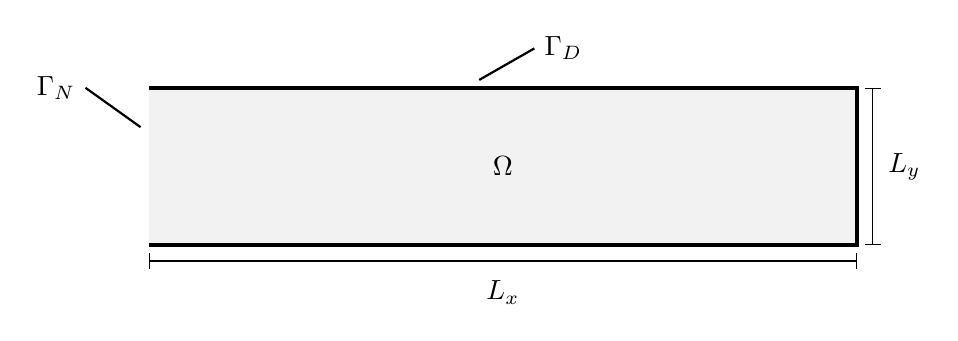
\begin{tikzpicture}
    \fill[black!5!white] (0, 0) rectangle (9, 2);
    \draw[ultra thick] (0, 0) to (9, 0) to (9, 2) to (0, 2);
    \draw[thick] (-0.8, 2) node[left] {$\Gamma_N$} to (-0.1, 1.5);
    \draw[thick] (4.9, 2.5) node[right] {$\Gamma_D$} to (4.2, 2.1);
    \draw[|-|] (0, -0.2) to (9, -0.2);
    \draw[|-|] (9.2, 0) to (9.2, 2);
    \node at (4.5, -0.6) {$L_x$};
    \node at (9.6, 1) {$L_y$};
    \node at (4.5, 1) {$\Omega$};
\end{tikzpicture}

    \caption{TODO.}
    \label{fig:rectangular_cavity}
\end{figure}

% Exploratory plots

% Rational interpolation demonstration
For $||\mathbf{u}||_{L_2(\Omega)}^2 = \int_{\Omega} ||\mathbf{u}||^2$

% Analytical and numerical root finding
Analytical eigenfrequencies
\begin{equation}
    \omega_{n, m} = \pi \sqrt{\left(\frac{2n + 1}{2L_x}\right)^2 + \left(\frac{m}{L_y}\right)^2},
    ~n \in \{0, 1, \dots\}, ~m \in \{1, 2, \dots \} \label{equ:analytical-eigenmodes}
\end{equation}
Numerical eigenfrequencies, solve generalized (symmetric) eigenvalue problem
\begin{equation}
    \mathbf{\underline{K}} \mathbf{u} = \omega^2 \mathbf{\underline{M}} \mathbf{u}
    \label{equ:numerical-eigenmodes}
\end{equation}
% maybe also talk about removing boundary indices

% Problems with non-resonant solutions suppressed by the boundary integral
Take $\{ \mathbf{u}_j, \omega_j^2 \}_j$ be the resonant modes, i.e. solutions to 
the eigenvalue problem (\ref{equ:numerical-eigenmodes}), such that
\begin{equation}
    \mathbf{\underline{K}} \mathbf{u}_j = \omega_j^2 \mathbf{\underline{M}} \mathbf{u}_j
    \label{equ:eigen-solution}
\end{equation}
Adding a source term $\mathbf{f}$ 
\begin{equation}
    \mathbf{\underline{K}} \mathbf{u} - \omega^2 \mathbf{\underline{M}} \mathbf{u} = \mathbf{f}
\end{equation}
If $\mathbf{u}$ is expressed in terms of the basis $\{ \mathbf{u}_j \}_j$, i.e.
$\mathbf{u} = \sum_j \alpha_j \mathbf{u}_j$
\begin{equation}
    \sum_j \alpha_j (\mathbf{\underline{K}} \mathbf{u}_j - \omega^2 \mathbf{\underline{M}} \mathbf{u}_j) = \mathbf{f}
\end{equation}
Using (\ref{equ:eigen-solution})
\begin{equation}
    \sum_j \alpha_j (\omega_j^2 - \omega^2) \mathbf{\underline{M}} \mathbf{u}_j = \mathbf{f}
\end{equation}
from which we can take the scalar product with $\mathbf{u}_j^H$ to obtain
% WHY SHOULD THIS BE A BASIS (DOES IT SPAN?), AND WHY M-ORTHONORMAL
\begin{equation}
    \alpha_j = \frac{\mathbf{u}_j^H \mathbf{f}}{\omega_j^2 - \omega^2}
\end{equation}
If $\mathbf{u}_j^H \mathbf{f} = 0$, then the resonant mode at $\omega_j$ is 
suppressed (fine with MRI, but eigsh will detect a resonant mode).

% Problems with linearly combinable solutions -> Use cubby to perturb waveguide
For $||\mathbf{u}||_{L_2(\Gamma)}^2 = \int_{\Gamma} ||\mathbf{u}||^2$

\subsection{Imperfectly conducting boundaries}
\label{subsec:examples-impedance}

% Numerical eigenfrequencies
Numerical eigenfrequencies, solve
\begin{equation}
    (\mathbf{\underline{K}} - i \omega \mathbf{\underline{I}} - \omega^2 \mathbf{\underline{M}}) \mathbf{u} = 0
\end{equation}
Define $\mathbf{v} = \omega \mathbf{u}$, so that we may write this as the
generalized eigenvalue problem
\begin{equation}
    \begin{bmatrix}
         & \boldsymbol{\underline{1}} \\
        \mathbf{\underline{K}} & -i \mathbf{\underline{I}}
    \end{bmatrix}
    \begin{bmatrix}
        \mathbf{u} \\
        \mathbf{v}
    \end{bmatrix}
    =
    \omega
    \begin{bmatrix}
        \boldsymbol{\underline{1}} & \\
         & \boldsymbol{\underline{M}}
    \end{bmatrix}
    \begin{bmatrix}
        \mathbf{u} \\
        \mathbf{v}
    \end{bmatrix}
\end{equation}
which is, however, no longer Hermitian (LHS chosen as \enquote{diagonal} as possible).
% Pole plot

\subsection{Dual mode circular waveguide filter}
\label{subsec:examples-dmcwf}

% Describe geometry and physical meaning

\begin{figure}[h]
    \centering
    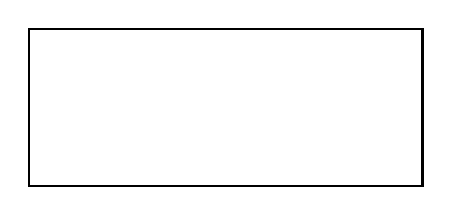
\begin{tikzpicture}
    \draw[thick] (0, 0) rectangle (5, 2);
\end{tikzpicture}
    \caption{Dual-mode circular waveguide filter. \cite{DMCWF-Dimensions}
    $W_C=43.87$ mm, $D_C=28.0$ mm, $L_B=43.87$ mm, $W_B=19.05$ mm, $H_B=9.525$ mm,
    $L_B=20.0$ mm, $W_S=10.05$ mm, $H_S=3.0$ mm, $W_A=2.0$ mm, $H_A=3.375$ mm,
    $L_A=2.825$ mm, thickness of all irises $2.0$ mm, screws half way up
    the cavity horizontal tuning screws with depth $3.82$ mm
    and coupling screws at angles $\pm 45^{\circ}$ with depth $3.57$ mm.}
    \label{fig:DMCWF}
\end{figure}

% Modeling process cite rubia

% Scattering coefficient

% Measurement procedure


\pagebreak
\section{Conclusion and outlook}
\label{sec:conclusion}

\pagebreak
\section{Appendix}
\label{sec:appendix}

\subsection{Detailed derivation for the weak formulation of the time-harmonic potential equation}
\label{subsec:derivation}

% !REMINDME: Levi-Civita tensor explanations.
The goal is to rewrite the curl-integral on the left-hand side of 
(\ref{equ:maxwell-weak-initial}):
\begin{equation}
    \int_{\Omega} (\nabla \times (\mu^{-1} \nabla \times \mathbf{u})) \cdot \mathbf{v} \label{equ:maxwell-weak-initial-LHS}
\end{equation}
In order to simplify the curls and apply the Gauss theorem, I first show
the following vector calculus identity:
\begin{fancybox}{Curl product rule}
    \begin{equation}
        (\nabla \times \mathbf{a}) \cdot \mathbf{b} = \nabla \cdot (\mathbf{a} \times \mathbf{b}) + \mathbf{a} \cdot (\nabla \times \mathbf{b}) \label{equ:vector-calculus} \\
    \end{equation}
\end{fancybox}
% !REMINDME: Appropriate spaces
where $\mathbf{a}$, $\mathbf{b}$ are vector-value functions. The completely
antisymmetric tensor $\varepsilon_{ijk}$, frequently referred to as the
Levi-Civita tensor, may be employed to rewrite the components of the
curl of a vector-function $\mathbf{a}$ as the sum
% !REMINDME: Maybe lemma and proof formatting
\begin{equation}
    (\nabla \times \mathbf{a})_k = \sum_i \sum_j \varepsilon_{ijk} \partial_i u_j
\end{equation}
where $\partial_i$ denotes the partial derivative with respect to the $i$-th coordinate
direction. This yields
\begin{align}
    (\nabla \times \mathbf{a}) \cdot \mathbf{b} &= \sum_k (\nabla \times \mathbf{a})_k b_k \notag \\ 
    &= \sum_k (\sum_i \sum_j \varepsilon_{ijk} \partial_i a_j) b_k \notag \\ 
    &= \sum_k \sum_i \sum_j \partial_i (\varepsilon_{ijk} a_j b_k) - \sum_k \sum_i \sum_j a_j (\varepsilon_{ijk} \partial_i b_k) \notag \\ 
    &= \sum_k \sum_i \sum_j \partial_i (\varepsilon_{jki} a_j b_k) - \sum_k \sum_i \sum_j a_j ((-\varepsilon_{ikj}) \partial_i b_k) \notag \\ 
    &= \sum_i \partial_i (\mathbf{a} \times \mathbf{b})_i + \sum_j u_j (\nabla \times \mathbf{b})_j \notag \\ 
    &= \nabla \cdot (\mathbf{a} \times \mathbf{b}) + \mathbf{a} \cdot (\nabla \times \mathbf{b}) \label{equ:curlidentity} 
\end{align}
by expressing the scalar product as a component-sum, using the product rule and
applying the symmetry and anti-symmetry properties of the Levi-Civita tensor.
Now the identity (\ref{equ:vector-calculus}) to (\ref{equ:maxwell-weak-initial-LHS})
together with Gauss' theorem gives
\begin{align}
    \int_{\Omega} (\nabla \times ({\mu^{-1} \nabla \times \mathbf{u}})) \cdot \mathbf{v} &=
    \int_{\Omega} \nabla \cdot (({\mu^{-1} \nabla \times \mathbf{u}}) \times \mathbf{v})
    + \int_{\Omega} ({\mu^{-1} \nabla \times \mathbf{u}}) \cdot (\nabla \times \mathbf{v}) \notag \\
    &= \int_{\partial \Omega} (({\mu^{-1} \nabla \times \mathbf{u}}) \times \mathbf{v}) \cdot \mathbf{n}
    + \int_{\Omega} ({\mu^{-1} \nabla \times \mathbf{u}}) \cdot (\nabla \times \mathbf{v}) \notag \\
\end{align}

For later convenience, the boundary integral can further be simplified using the
\begin{fancybox}{Commutative behavior of the scalar triple product}
    \begin{equation}
        (\mathbf{a} \times \mathbf{b}) \cdot \mathbf{c} = - (\mathbf{a} \times \mathbf{c}) \cdot \mathbf{b} \label{equ:vector-algebra}
    \end{equation}
\end{fancybox}
This identity follows immediately from a small manipulation with the Levi-Civita
tensor:
\begin{align}
    (\mathbf{a} \times \mathbf{b}) \cdot \mathbf{c} &= \sum_k (\sum_i \sum_j \varepsilon_{ijk} a_i b_j) c_k \notag \\
     &= \sum_j (\sum_i \sum_k (-\varepsilon_{ikj}) a_i c_k) b_j \notag \\ 
     &= - (\mathbf{a} \times \mathbf{c}) \cdot \mathbf{b} 
\end{align}
The boundary integral becomes 
\begin{equation}
    \int_{\partial \Omega} (({\mu^{-1} \nabla \times \mathbf{u}}) \times \mathbf{v}) \cdot \mathbf{n}
    = - \int_{\partial \Omega} (({\mu^{-1} \nabla \times \mathbf{u}}) \times \mathbf{n}) \cdot \mathbf{v}
\end{equation}

This concludes the short derivation, because now (\ref{equ:maxwell-weak-initial-LHS})
may be rewritten as
\begin{equation}
    - \int_{\partial \Omega} (({\mu^{-1} \nabla \times \mathbf{u}}) \times \mathbf{v}) \cdot \mathbf{n}
    + \int_{\Omega} ({\mu^{-1} \nabla \times \mathbf{u}}) \cdot (\nabla \times \mathbf{v})
\end{equation}

% 
\newpage
\bibliography{biblio.bib}

\end{document}